\begin{figure}
    \begin{center}
        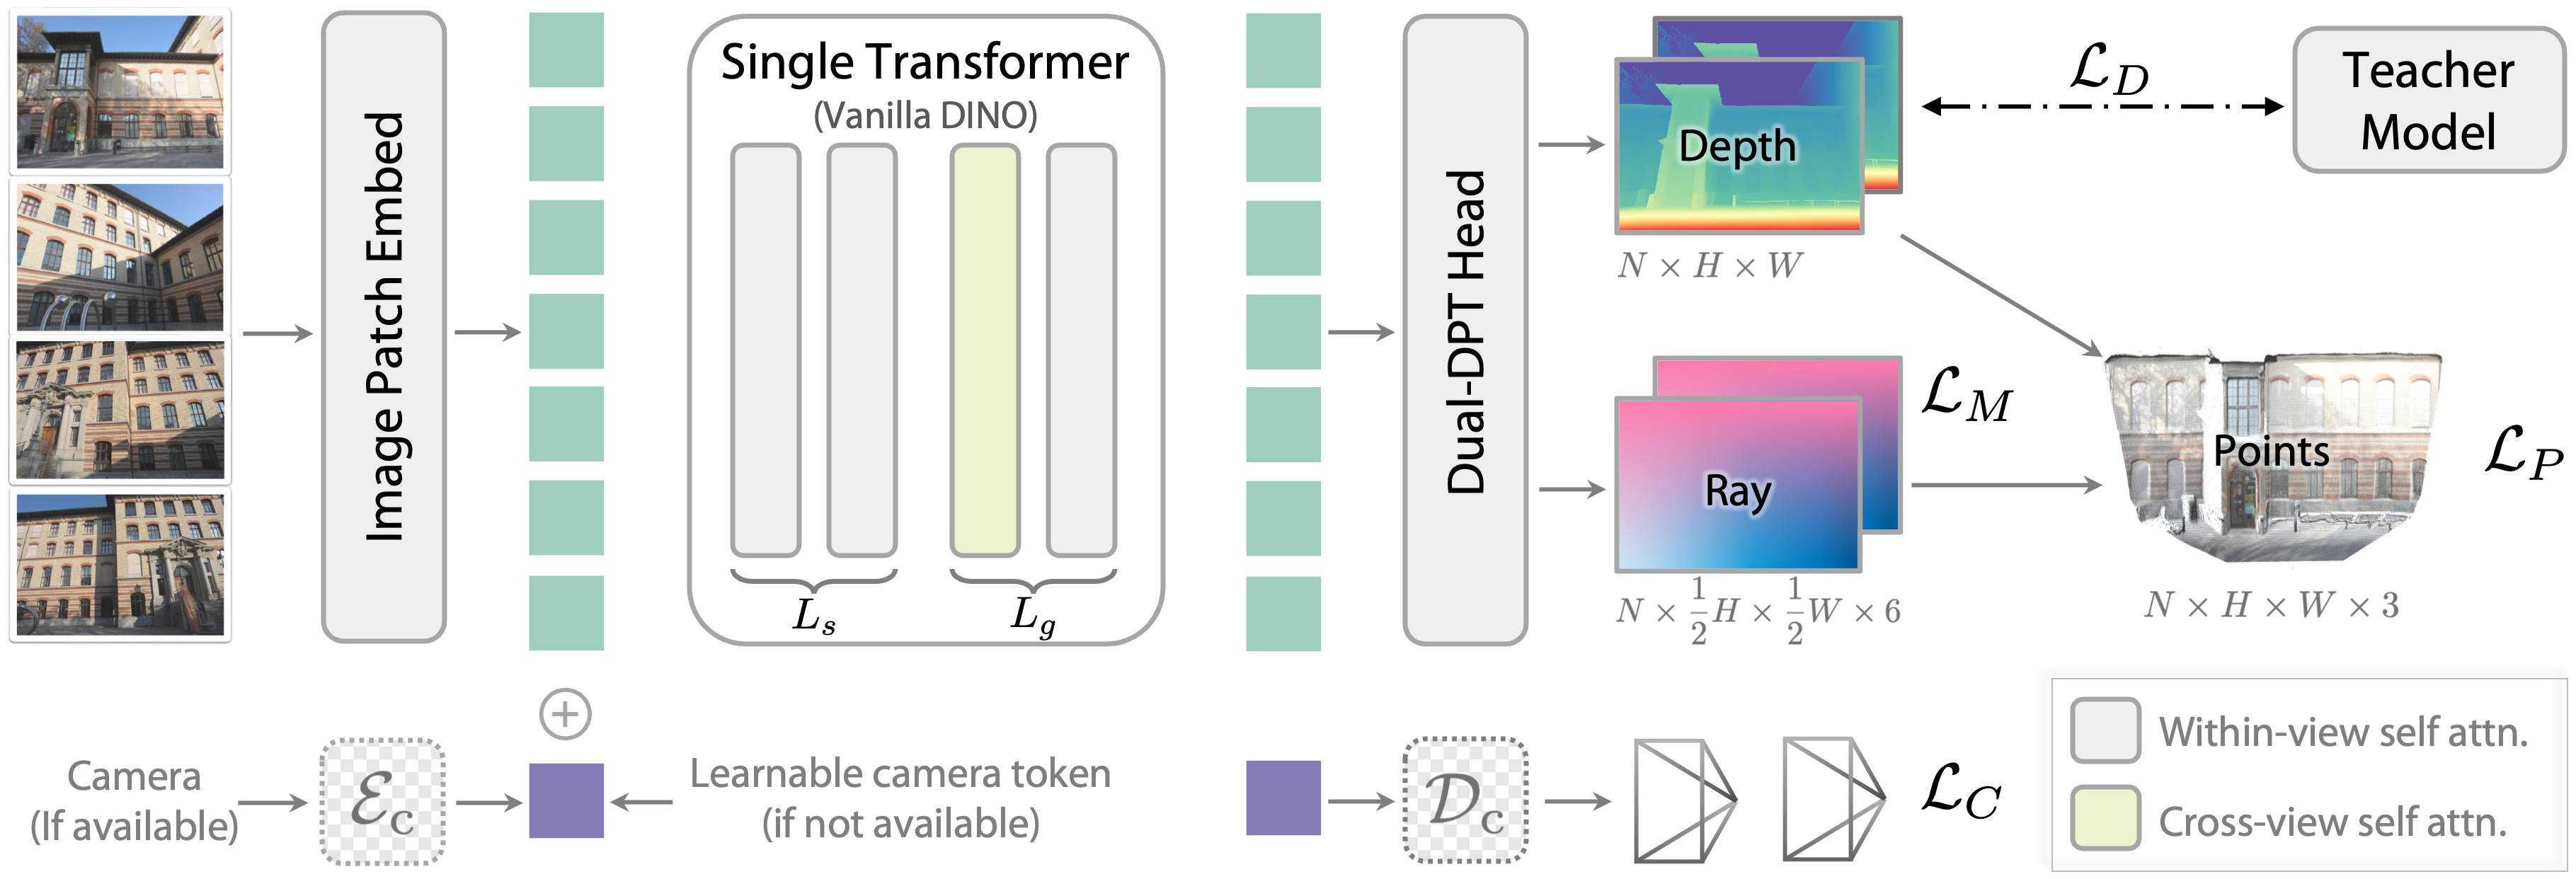
\includegraphics[width=0.95\textwidth]{figs/pdfs/pipeline.png}
        \caption{\textbf{Pipeline of Depth Anything 3.} 
        Depth Anything 3 employs a single transformer (vanilla DINOv2 model) without any architectural modifications. To enable cross-view reasoning, an input-adaptive cross-view self-attention mechanism is introduced. A dual-DPT head is used to predict depth and ray maps from visual tokens.
        Camera parameters, if available, are encoded as camera tokens and concatenated with patch tokens, participating in all attention operations.  
        }
        \label{fig:pipeline}
    \end{center}
\end{figure}


\section{Depth Anything 3}
\label{sec:method}


我们致力于从多样的视觉输入——单张图像、多视图集合或视频——中恢复一致的3D几何结构，并在已知相机位姿可用时可选地融入这些信息。

\subsection{问题形式化}
\label{sec:formulation}


我们将输入记为 $\inputset=\{\inputimage_i\}_{i=1}^{N_v}$，其中每个 $\inputimage_i \in \mathbb{R}^{H \times W \times 3}$。当 $N_v=1$ 时为单目图像，当 $N_v>1$ 时则代表视频或多视图集合。每幅图像对应深度 $\depthmap_i \in \mathbb{R}^{H \times W}$、相机外参 $\big[\camerarot_i \mid \cameratrans_i\big]$ 和内参 $\cameraint_i$。相机也可表示为 $\cameravec_i \in \mathbb{R}^9$，包含平移 $\cameratrans_i\in \mathbb{R}^3$、旋转四元数 $\rotquat_i\in \mathbb{R}^4$ 和视场角参数 $\fovparam_i\in \mathbb{R}^2$。像素 $\pixelcoord=(u,v,1)^\top$ 投影到3D点 $\worldpoint=(X,Y,Z,1)^\top$ 的过程为：
\begin{equation*}
    \worldpoint=\camerarot_i\big(\depthmap_i(u,v)\,\cameraint_i^{-1}\pixelcoord\big)+\cameratrans_i,
\end{equation*}
通过该投影，底层的3D视觉空间可以被忠实地恢复。



\paragraph{深度-射线表示。} 预测有效的旋转矩阵 $\mathbf{R}_i$ 因正交约束而具有挑战性。为规避这一问题，我们使用逐像素的射线图隐式表示相机位姿，该射线图与输入图像和深度图对齐。对于每个像素 $\pixelcoord$，相机射线 $\cameraray \in \mathbb{R}^6$ 由其原点 $\rayorigin \in \mathbb{R}^3$ 和方向 $\raydir \in \mathbb{R}^3$ 定义：$\cameraray = (\rayorigin, \raydir)$。方向通过将 $\pixelcoord$ 反投影到相机坐标系并旋转至世界坐标系得到：
$
    \raydir = \camerarot \cameraint^{-1} \pixelcoord.
$
稠密射线图 $\raymap \in \mathbb{R}^{H \times W \times 6}$ 存储所有像素的这些参数。我们不对 $\raydir$ 进行归一化，因此其幅度保留了投影尺度。由此，世界坐标系中的3D点可简单地表示为：
$
    {\worldpoint} = {\rayorigin} + \depthmap(u, v) \cdot \raydir.
    \label{eq:depth_to_pcd}
$
该形式化通过将预测的深度图和射线图进行逐元素操作，能够生成一致的点云。





\label{sec:ray2pose}
\paragraph{从射线图推导相机参数。}
给定输入图像 $\inputimage \in \mathbb{R}^{H\times W \times 3}$，对应的射线图记为 $\raymap \in \mathbb{R}^{H \times W \times 6}$。该图包含逐像素的射线原点（存储在前三个通道 $\raymap(:,:,:3)$）和射线方向（存储在后三个通道 $\raymap(:,:,3:)$）。

首先，相机中心 $\rayorigin_c$ 通过对逐像素射线原点向量取平均来估计：
\begin{equation}
    \rayorigin_c = \frac{1}{H \times W} \sum_{h=1}^{H}\sum_{w=1}^W \raymap(h, w, :3).
\end{equation}

为了估计旋转 $\camerarot$ 和内参 $\cameraint$，我们将问题形式化为求解一个单应矩阵 $\mathbf{H}$。
我们首先定义一个具有单位内参矩阵的"单位"相机，$\cameraint_I = \mathbf{I}$。
对于给定像素 $\pixelcoord$，其在该标准相机坐标系中的对应射线方向即为 $\mathbf{d}_I = \cameraint_I^{-1} \pixelcoord = \pixelcoord$。
从该标准射线 $\mathbf{d}_I$ 到目标相机坐标系中射线方向 $\mathbf{d}_\text{cam}$ 的变换为 $\mathbf{d}_\text{cam} = \cameraint \camerarot \mathbf{d}_I$。
这就在两组射线之间建立了一个直接的单应关系 $\mathbf{H} = \cameraint \camerarot$。
然后，我们通过最小化变换后的标准射线与预计算的目标射线 $\raymap(h,w,3:)$ 之间的几何误差来求解该单应矩阵。这引出以下优化问题：
\begin{equation}
    \mathbf{H}^* = \arg\min_{||\mathbf{H}|| = 1}\sum_{h=1}^{H}\sum_{w=1}^W \left|\left| \mathbf{H} \pixelcoord_{h,w} \times \raymap(h,w,3:) \right|\right|.
\end{equation}
这是一个标准的最小二乘问题，可以使用直接线性变换（DLT）算法~\citep{abdel2015direct} 高效求解。
一旦找到最优单应矩阵 $\mathbf{H}^*$，我们便可恢复相机参数。
由于内参矩阵 $\cameraint$ 是上三角矩阵而旋转矩阵 $\camerarot$ 是正交矩阵，我们可以对 $\mathbf{H}^*$ 进行RQ分解来唯一地分解出 $\cameraint$ 和 $\camerarot$。

\paragraph{最小预测目标集。} 近期工作致力于构建统一的3D任务模型，通常采用多任务学习并使用不同的预测目标——例如，单独的点图~\citep{dust3r}，或位姿、局部/全局点图和深度的冗余组合~\citep{wang2025vggt,cut3r,fast3r}。点图不足以确保一致性，而冗余目标虽能提升位姿精度，但常引入耦合而损害位姿估计。
相比之下，我们的实验（\cref{tab:ablation_minimal_targets}）表明，深度-射线表示构成了同时捕捉场景结构和相机运动的最小且充分的目标集，其表现优于点图或更复杂输出等替代方案。
然而，在推理时从射线图恢复相机位姿计算成本较高。为此，我们增加了一个轻量级的相机头 $\camerahead$。该Transformer在相机令牌上操作，用于预测视场角（$\fovparam \in \mathbb{R}^2$）、旋转四元数（$\rotquat \in \mathbb{R}^4$）和平移（$\cameratrans \in \mathbb{R}^3$）。由于每视图仅处理一个令牌，增加的计算开销可忽略不计。















\subsection{网络架构} \label{sec:archi}
下面我们详细介绍Depth Anything 3的网络架构，如 \cref{fig:pipeline} 所示。该网络由三个主要组件构成：一个作为骨干网络的单一Transformer模型、一个用于位姿条件化的可选相机编码器，以及一个用于生成预测结果的双DPT预测头。

\textbf{单一Transformer骨干网络。} 我们使用具有 $\transformerlayers$ 个块的视觉Transformer，并在大规模单目图像语料库（如DINOv2~\cite{oquab2023dinov2}）上进行预训练。
通过一种输入自适应的自注意力机制，对输入令牌进行重新排列，可以在不改变网络架构的情况下实现跨视角推理。
我们将Transformer分为两组，大小分别为 $\singleviewlayers$ 和 $\globallayers$。
前 $\singleviewlayers$ 层在每幅图像内部应用自注意力，而后面的 $\globallayers$ 层在跨视角和视角内注意力之间交替切换，通过张量重排序在所有令牌上联合操作。
实际中，我们设置 $\singleviewlayers:\globallayers = 2:1$，其中 $\transformerlayers = \singleviewlayers + \globallayers$。
如 \cref{tab:abl_dav3} 中的消融研究所示，与其他配置相比，这一设置在性能和效率之间提供了最优权衡。
该设计是输入自适应的：当输入为单张图像时，模型自然地退化为单目深度估计，无需额外开销。





\textbf{相机条件注入。}
为了无缝处理既有位姿和无位姿的输入，我们为每个视图预置一个相机令牌 $\cameratoken_i$。
如果相机参数 $(\cameraint_i, \camerarot_i, \cameratrans_i)$ 可用，则通过一个轻量级MLP $\cameraencoder$ 获得该令牌：$\cameratoken_i = \cameraencoder(\fovparam_i, \rotquat_i, \cameratrans_i)$。
否则，使用一个共享的可学习令牌 $\learnabletoken$。
这些相机令牌与图像块令牌拼接在一起，参与所有注意力操作，提供显式的几何上下文或一致的可学习占位信息。



\begin{wrapfigure}{r}{0.5\textwidth}
    \centering
    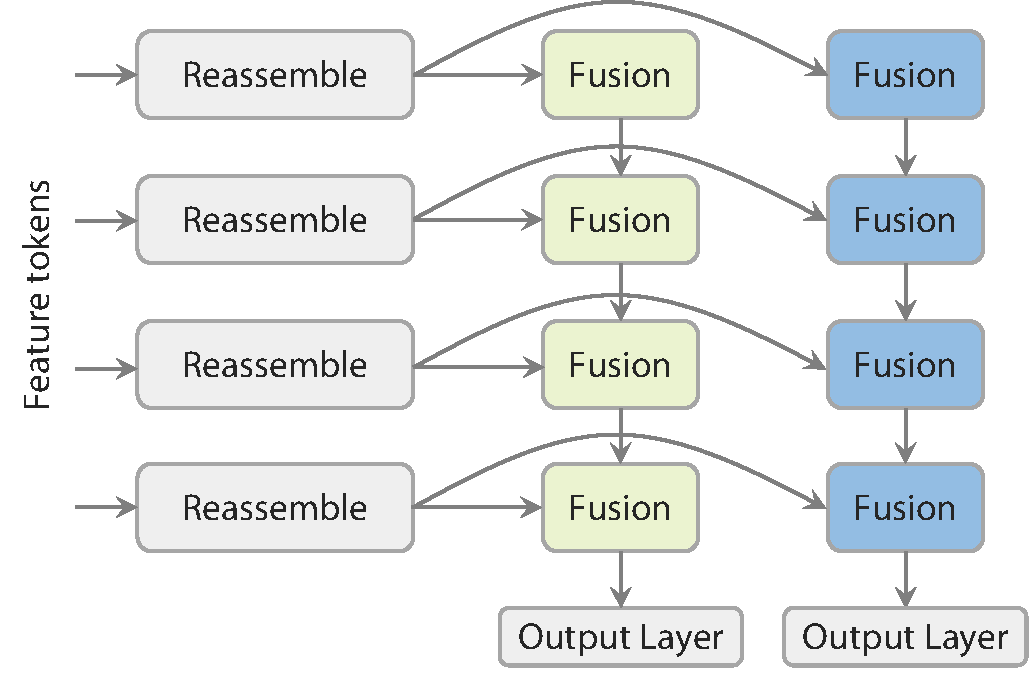
\includegraphics[width=0.48\textwidth]{figs/pdfs/dual_dpt.pdf}
    \caption{\textbf{双DPT预测头。} 两个分支共享重组装模块以实现更好的输出对齐。}
    \label{fig:wrap_example}
\end{wrapfigure}


\textbf{双DPT预测头。}
在最终预测阶段，我们提出了一种新颖的双DPT预测头，联合生成稠密的深度值和射线值。如 \cref{tab:ablation_minimal_targets} 所示，该设计既强大又高效。给定来自骨干网络的一组特征，双DPT预测头首先通过一组共享的重组装模块对它们进行处理。随后，处理后的特征通过两组不同的融合层进行融合：一组用于深度分支，一组用于射线分支。最后，两个独立的输出层生成最终的深度图和射线图预测。该架构确保两个分支在相同的处理特征集上操作，仅在最后的融合阶段有所不同。这种设计促进了两个预测任务之间的强交互，同时避免了冗余的中间表示。





\subsection{训练} \label{sec:training}


\textbf{教师-学生学习范式。}
我们的训练数据来自多种来源，包括真实世界的深度采集数据、3D重建数据和合成数据集。
真实世界的深度数据通常带有噪声且不完整（\cref{fig:poordataset}），这限制了其监督价值。
为解决这一问题，我们训练了一个仅使用合成数据的单目相对深度估计"教师"模型，用于生成高质量的伪标签。
这些伪深度图通过RANSAC最小二乘法与原始的稀疏或带噪声的标注真值对齐，在保持几何精度的同时增强了标签的细节和完整性。
我们将该模型称为Depth-Anything-3-Teacher，它在涵盖室内、室外、以物体为中心以及多种野外场景的大规模合成语料库上训练，以捕获精细几何结构。
我们在~\cref{sec:teacher}中详细介绍了教师模型的设计。



\newcommand{\errd}{e^{\mathrm{D}}}
\newcommand{\nz}{Z_{\Omega}}

\paragraph{训练目标。}
遵循 \cref{sec:formulation} 中的形式化，
我们的模型 $\model$ 将输入 $\inputset$ 映射到一组输出，包括深度图 $\preddepth$、射线图 $\predray$ 以及可选的相机位姿 $\textcolor{gray}{\predcamera}$：
$\model: \inputset \mapsto \{\preddepth, \predray, \textcolor{gray}{\predcamera}\}$。
灰色表示 $\textcolor{gray}{\predcamera}$ 是可选输出，主要出于实际便利而包含。在计算损失之前，所有标注真值信号均通过一个公共尺度因子进行归一化。该尺度定义为有效的重投影点图 $\worldpoint$ 的平均 $\ell_{2}$ 范数，这一步骤确保了不同模态之间的量级一致，并稳定了训练过程。总体训练目标定义为若干项的加权和：
\begin{equation*}
\totalloss = \depthloss(\preddepth, \depthmap) + \rayloss(\predray, \raymap) + \pointloss(\preddepth \odot \raydir + \rayorigin, \worldpoint) + \textcolor{gray}{\cameraweight \cameraloss (\predcamera, \cameravec)}
+ \gradweight \gradloss(\preddepth, \depthmap),
\label{eq:loss}
\end{equation*}
\begin{equation*}
    \depthloss(\preddepth, \depthmap \,;\, D_c)
    = \tfrac{1}{\nz} \sum_{p \in \Omega} m_p \left( D_{c,p}\, \big|\preddepth_p - \depthmap_p\big| - \lambda_c \log D_{c,p} \right),
\end{equation*}
其中 $D_{c,p}$ 表示深度 $D_p$ 的置信度。所有损失项均基于 $\ell_{1}$ 范数，权重设置为 $\gradweight=1$ 和 $\cameraweight=1$。梯度损失 $\gradloss$ 对深度梯度进行惩罚：
\begin{equation}
\gradloss(\preddepth, \depthmap) = ||\gradx \preddepth - \gradx \depthmap||_{1} + ||\grady \preddepth - \grady \depthmap||_{1},
\end{equation}
其中 $\gradx$ 和 $\grady$ 分别是水平和垂直方向的有限差分算子。该损失在保持锐利边缘的同时确保平坦区域的平滑性。
实际中，我们设置 $\alpha=1$ 和 $\beta = 1$。

\subsection{实现细节}

\paragraph{训练数据集。}
我们在表~\ref{tab:datasets}中提供了训练数据集。
需要注意的是，对于训练集和测试集之间可能存在重叠的数据集（如ScanNet++），我们在场景级别确保严格的分离，即训练和测试中的场景互斥。使用ScanNet++进行训练对其他方法是公平的，因为它在~\cite{wang2025vggt,dust3r}中被广泛用于训练。
\begin{table}[ht]
\centering
\caption{\longname{}使用的数据集，包括场景数量和数据类型。}
\label{tab:datasets}
\begin{tabular}{l|llc}
\toprule
\textbf{Usage} & \textbf{Dataset} & \textbf{\#Scenes} & \textbf{Data Type} \\
\midrule
\multirow{5}{*}{\makecell{Pose-geometry \\ benchmark}} 
  & HiRoom (ours)        & 29  & Synthetic \\
  & ETH3D~\citep{schops2017eth3d}     & 11  & LiDAR \\
  & DTU~\citep{aanaes2016dtu}         & 22  & LiDAR \\
  & 7Scenes~\citep{shotton2013sevenscene} & 7   & LiDAR \\
  & ScanNet++~\citep{yeshwanth2023scannet++} & 20  & LiDAR \\
\midrule
\multirow{21}{*}{\makecell{Pose-geometry \\ Training}}
  & AriaDigitalTwin~\citep{pan2023aria} & 237   & Synthetic \\
  & AriaSyntheticENV~\citep{pan2023aria} & 99950  &  Synthetic \\
  & ArkitScenes~\citep{baruch2021arkitscenes}      & 4388 & LiDAR \\
  & BlendedMVS~\citep{yao2020blendedmvs} & 503 & 3D Recon \\
  & Co3dv2~\citep{reizenstein2021common} & 30616 & Colmap\\
  & DL3DV~\citep{ling2024dl3dv} & 6379 & Colmap \\
  & HyperSim~\citep{roberts2021hypersim} & 344 & Synthetic \\
  & MapFree~\citep{arnold2022map} & 921 & Colmap \\
  & MegaDepth~\citep{li2018megadepth} & 268 & Colmap \\ 
  & MegaSynth~\citep{jiang2025megasynth} & 6049 & Synthetic \\ 
  & MvsSynth~\citep{DeepMVS} & 121 & Synthetic \\
  & Objaverse~\citep{deitke2023objaverse} & 505557 & Synthetic \\ 
  & Omniobject~\citep{wu2023omniobject3d} & 5885 & Synthetic\\ 
  & OmniWorld~\citep{zhou2025omniworld} & 1039 & Synthetic\\ 
  & PointOdyssey~\citep{zheng2023pointodyssey} & 44 & Synthetic \\ 
  & ReplicaVMAP~\citep{straub2019replica} & 17 & Synthetic \\
  & ScanNet++~\citep{yeshwanth2023scannet++} & 230 & LiDAR \\
  & ScenenetRGBD~\citep{mccormac2017scenenet} & 16866 & Synthetic \\
  & TartanAir~\citep{tartanair2020iros} & 355 & Synthetic \\
  & Trellis~\citep{xiang2024structured} & 557408 & Synthetic \\
  & vKitti2~\citep{cabon2020vkitti2} & 50 & Synthetic \\
  & WildRGBD~\citep{xia2024rgbd} & 23050 & LiDAR \\
\bottomrule
\end{tabular}

\end{table}



\paragraph{训练细节。}
我们在128块H100 GPU上训练模型共20万步，使用8千步的预热阶段和峰值学习率 $2 \times10^{-4}$。
基础分辨率为 $504\times504$，该数值能被2、3、4、6、9和14整除，使其与常见的照片宽高比（如2:3、3:4和9:16）更加兼容。
训练图像分辨率从以下值中随机采样：$504\times504$、$504\times378$、$504\times336$、$504\times280$、$336\times504$、$896\times504$、$756\times504$、$672\times504$。对于 $504\times504$ 分辨率，视图数量从 [2, 18] 中均匀采样。批量大小动态调整，以保持每步的令牌数量大致恒定。在12万步时，监督信号从标注真值深度切换为教师模型标签。位姿条件化在训练期间以0.2的概率随机激活。







\section{教师-学生学习}
\begin{wrapfigure}{r}{0.5\textwidth} 
    \vspace{-5mm}
    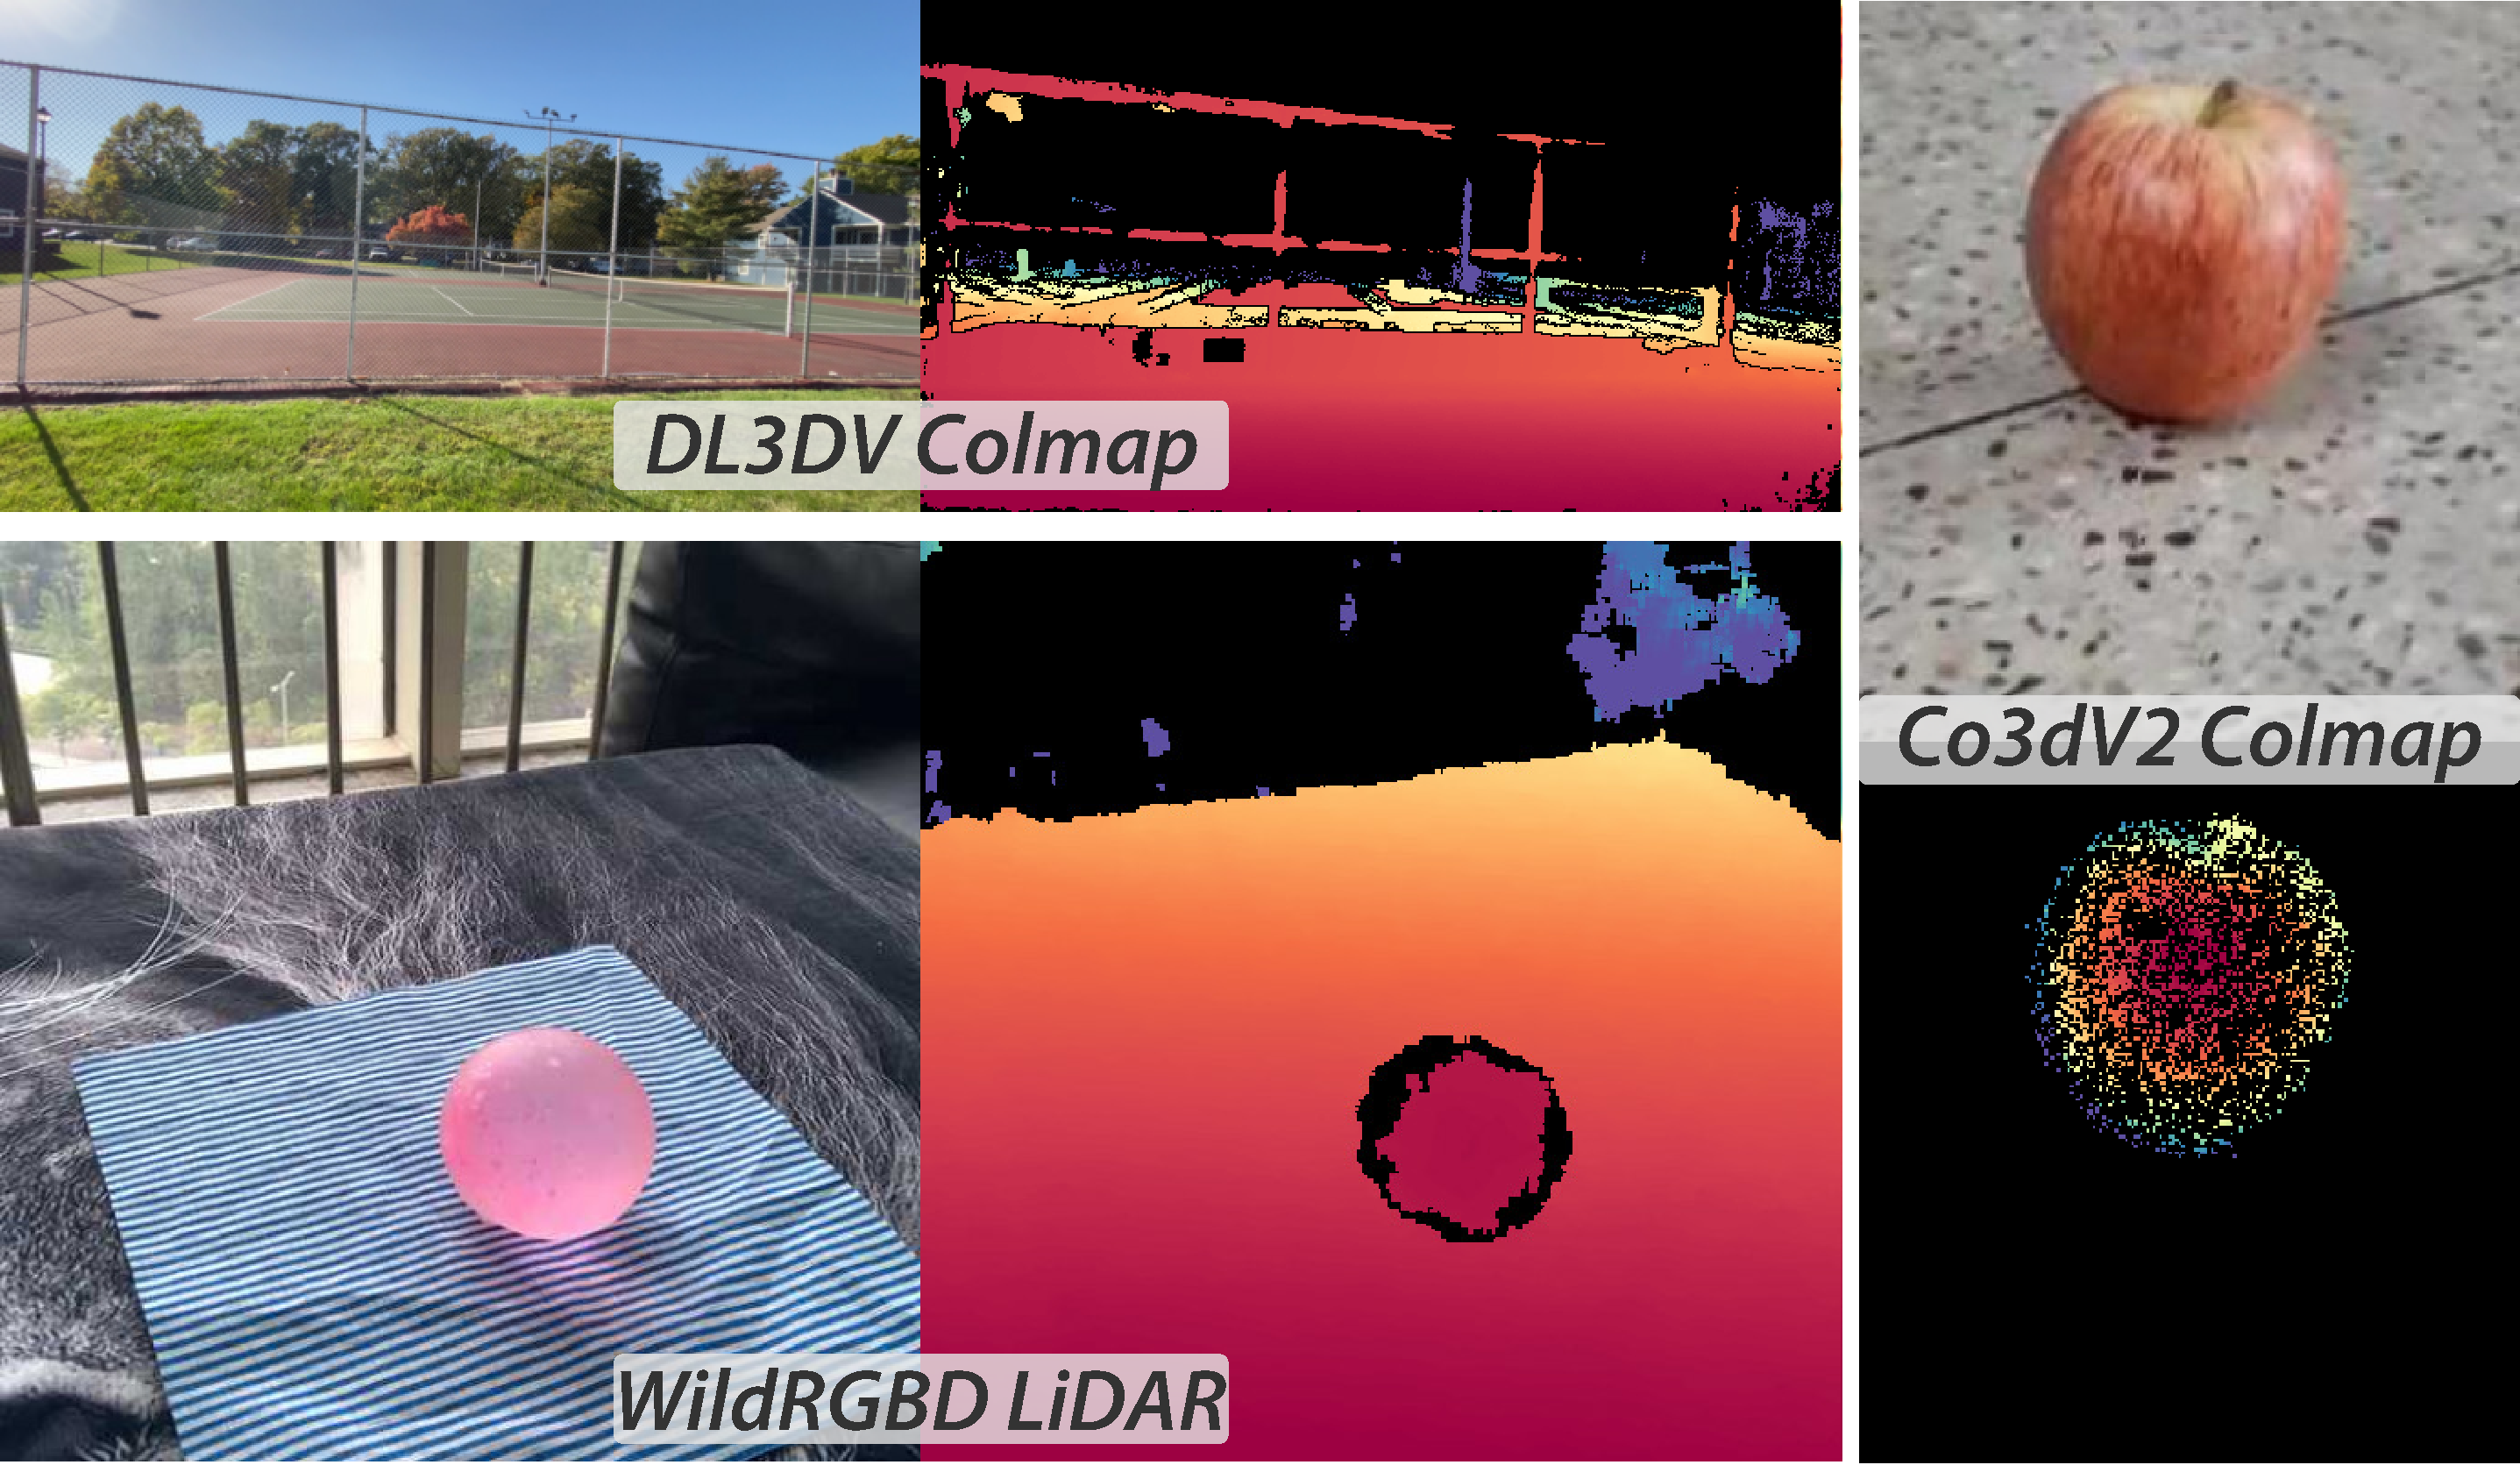
\includegraphics[width=0.48\textwidth]{figs/pdfs/dataset.pdf}
    \caption{\textbf{Poor quality real-world datasets.} We show some examples of the poor quality real-world datasets. }
    \label{fig:poordataset}
    \vspace{-8mm}
\end{wrapfigure}




如~\cref{fig:poordataset}所示，真实世界数据集的质量较差，因此我们仅在合成数据上训练教师模型，为真实世界数据提供监督。
我们的教师模型作为单目相对深度预测器进行训练。在推理或提供监督时，带噪声的标注真值深度可用于提供尺度和偏移参数，从而将预测的相对深度与绝对深度测量值对齐。

\subsection{构建教师模型} \label{sec:teacher}

在Depth Anything 2~\cite{yang2024depth}的基础上，我们在包括数据和表示在内的多个关键方面进行了扩展。我们观察到，扩大训练语料库能显著提升深度估计性能，验证了数据规模化的益处。此外，虽然我们改进的深度表示在标准的2D评估指标上可能没有显著提升，但它能产生质量更优的3D点云，展现出更少的几何畸变和更真实的场景结构。
需要注意的是，我们的教师网络骨干结构与上述DA3框架直接对齐，仅由DINOv2视觉Transformer和DPT解码器组成——没有引入专门的架构修改。我们在以下各节中详细阐述完整的设计和实现细节。


\noindent{\bf 数据规模化。} 我们仅在合成数据上训练教师模型，以获得更精细的几何细节。DA2中使用的合成数据集相对有限。在DA3中，我们大幅扩展了训练语料库，包括：Hypersim~\citep{roberts2021hypersim}、TartanAir~\citep{tartanair2020iros}、IRS~\citep{wang2019irs}、vKITTI2~\citep{cabon2020vkitti2}、BlendedMVS~\citep{yao2020blendedmvs}、SPRING~\citep{mehl2023spring}、MVSSynth~\citep{DeepMVS}、UnrealStereo4K~\citep{zhang2018unrealstereo}、GTA-SfM~\citep{wang2020flow}、TauAgent~\citep{gil2021online}、KenBurns~\cite{niklaus20193d}、MatrixCity~\citep{li2023matrixcity}、EDEN~\citep{le2021eden}、ReplicaGSO~\citep{replica19arxiv}、UrbanSyn~\citep{GOMEZ2025130038}、PointOdyssey~\citep{zheng2023pointodyssey}、Structured3D~\citep{zheng2020structured3d}、Objaverse~\citep{deitke2023objaverse}、Trellis~\citep{xiang2024structured}和OmniObject~\citep{wu2023omniobject3d}。这一集合涵盖了室内、室外、以物体为中心以及多种野外场景，提升了教师模型的泛化能力。

\noindent{\bf 深度表示。} 与DA2预测尺度-偏移不变的视差不同，我们的教师模型输出的是尺度-偏移不变的深度。深度更有利于下游任务，如度量深度估计和多视图几何，这些任务直接在深度空间而非视差空间中进行操作。
为解决深度相对于视差在近相机区域灵敏度较低的问题，我们预测指数深度而非线性深度，从而增强对小距离的分辨能力。

\noindent{\bf 训练目标。}
在几何监督方面，除了标准的深度-梯度损失外，我们还采用~\cite{wang2025moge}中引入的全局-局部损失进行ROE对齐。为进一步优化局部几何结构，我们引入了距离加权的表面法向损失。对于每个中心像素，我们采样四个相邻点并计算未归一化的法向量 $n_i$。然后按以下方式对这些法向量加权：
\begin{equation}
  w_i= \sum _ {j=0}^ 4 \parallel n_j\parallel - \parallel n_i \parallel,
  \label{eq:normal_weight}
\end{equation}
该加权方式降低了远离中心的相邻点的贡献，使得平均法向量更接近真实的局部表面法向量：
\begin{equation}
 n_m= \sum _ {i=0}^ {4} w_i \frac {n_i}{\parallel n_i \parallel},
 \label{eq:normal_mean}
\end{equation}
最终的法向损失为：
\begin{equation}
 \mathcal{L}_{N} = \mathcal{E}(\hat{n}_{m}, n_m) + \sum _ {i=0}^{4} \mathcal{E}(\hat{n}_i, n_i)
 \label{eq:normal_loss}
\end{equation}
其中 $\mathcal{E}$ 表示法向量之间的角度误差。在天空区域以及仅含物体的数据集的背景区域中，标注真值是未定义的。为防止这些区域降低深度预测质量并便于下游使用，我们联合预测一个与深度输出对齐的天空掩码和一个物体掩码，使用MSE损失进行监督。总体训练目标为：
\begin{equation}
 \mathcal{L}_{T} = \gradweight \mathcal{L}_\text{grad} + \mathcal{L}_\text{gl} + \mathcal{L}_{N} + \mathcal{L}_\text{sky} + \mathcal{L}_\text{obj}
 \label{eq:teacher_loss}
\end{equation}
其中 $\gradweight = 0.5$。这里，$\mathcal{L}_\text{grad}$、$\mathcal{L}_\text{gl}$、$\mathcal{L}_\text{sky}$ 和 $\mathcal{L}_\text{obj}$ 分别表示梯度损失、全局-局部损失、天空掩码损失和物体掩码损失。

\subsection{教导Depth Anything 3}
真实世界数据集对于泛化相机位姿估计至关重要，但它们很少提供干净的深度数据；监督信号通常带有噪声或是稀疏的（\cref{fig:poordataset}）。Depth Anything 3 Teacher提供高质量的相对深度，我们通过鲁棒的RANSAC尺度-偏移过程将其与带噪声的度量深度（例如来自COLMAP或主动传感器的数据）对齐。设 \(\tilde{\depthmap}\) 为教师模型的相对深度，\(\depthmap\) 为可用的稀疏深度，并在区域 \(\Omega\) 上有有效性掩码 \(m_p\)。我们通过RANSAC最小二乘法估计尺度 \(s\) 和偏移 \(t\)，内点阈值设置为残差中位数的平均绝对偏差：
\begin{equation}
    (\hat{s},\hat{t})
    = \arg\min_{s>0,\,t} \sum_{p\in\Omega} m_p\,\big( s\,\tilde{\depthmap}_p + t - \depthmap_p\big)^2,\quad
    \depthmap^{T\rightarrow M} = \hat{s}\,\tilde{\depthmap} + \hat{t}.\label{eq:ss_align}
\end{equation}
对齐后的 \(\depthmap^{T\rightarrow M}\) 为Depth Anything 3提供了尺度一致且位姿-深度协调的监督，补充了我们的联合深度-射线训练目标，并提升了真实世界的泛化能力，如 \cref{fig:vis_teacher_sup} 所示。



\subsection{教导单目模型}

我们还以教师-学生范式额外训练了一个单目深度模型。
我们遵循DA2框架，在无标注图像上使用教师模型生成的伪标签来训练单目学生模型。与DA2的主要区别在于预测目标：我们的学生模型预测深度图，而DA2预测视差。我们进一步使用与教师模型相同的损失函数对学生模型进行监督，该损失应用于伪深度标签。
该单目模型也预测相对深度。仅使用无标注数据并在教师模型的监督下训练，该模型在标准单目深度基准上取得了最先进的性能，如 \cref{tab:student_mono} 所示。


\subsection{教导度量深度模型}
接下来，我们展示教师模型可用于训练具有锐利边界的度量深度估计模型。遵循Metric3Dv2~\cite{hu2024metric3dv2}，我们应用标准相机空间变换来解决由焦距变化引起的深度歧义。具体而言，我们使用比率 $f^c/f$ 对标注真值深度进行重新缩放，其中 $f^c$ 和 $f$ 分别表示标准焦距和相机焦距。为确保锐利细节，我们使用教师模型的预测作为训练标签。我们将教师模型预测深度的尺度和偏移与标注真值的度量深度标签对齐，以进行监督。

\paragraph{训练数据集。}
我们在14个数据集上训练度量深度模型，包括Taskonomy~\cite{zamir2018taskonomy}、DIML (Outdoor)~\cite{cho2021diml}、DDAD~\cite{ddad}、Argoverse~\cite{wilson2023argoverse}、Lyft~[]、PandaSet~\cite{xiao2021pandaset}、Waymo~\cite{Sun_2020_CVPR}、ScanNet++~\cite{yeshwanth2023scannet++}、ARKitScenes~\cite{baruch2021arkitscenes}、Map-free~\cite{arnold2022map}、DSEC~\cite{Gehrig21ral}、Driving Stereo~\cite{yang2019drivingstereo}和Cityscapes~\cite{cordts2016cityscapes}。对于立体数据集，我们利用FoundationStereo~\cite{wen2025foundationstereo}的预测作为训练标签。

\paragraph{实现细节。}
训练过程大致遵循单目教师模型的训练方式。所有图像在基础分辨率504下训练，具有多种宽高比（1:1、1:2、16:9、9:16、3:4、1:1.5、1.5:1、1:1.8）。我们使用AdamW优化器，编码器和解码器的学习率分别设置为5e-6和5e-5。我们应用随机旋转数据增强，训练图像以5\%的概率旋转90度或270度。标准焦距 $f^c$ 设置为300。我们使用教师模型的对齐预测作为监督。以20\%的概率，我们使用原始标注真值标签进行训练。批量大小为64，训练16万次迭代。训练目标是深度损失 $\mathcal{L}_{depth}$、$\mathcal{L}_{grad}$ 和天空掩码损失 $\mathcal{L}_{sky}$ 的加权和。


\section{应用：前馈式3D高斯泼溅}
\subsection{位姿条件化的前馈式3DGS}
受人类空间智能的启发，我们相信一致的深度估计可以极大地促进下游3D视觉任务。我们选择前馈式新视角合成（FF-NVS）作为演示任务，因为它在神经3D表示（即我们选择3DGS）的推动下日益受到关注，并且与众多应用场景相关。遵循最小化建模策略，我们通过微调一个添加的DPT头（GS-DPT）来推断逐像素对齐的3D高斯~\cite{charatan2024pixelsplat,chen2024mvsplat}，从而实现FF-NVS。

\textbf{GS-DPT头。}
给定通过我们的单一Transformer骨干网络（\cref{sec:archi}）提取的每个视图的视觉令牌，GS-DPT预测相机空间中的3D高斯参数 $\{ \sigma_i, \mathbf{q}_i, \mathbf{s}_i, \mathbf{c}_i \}_{i=1}^{H \times W} $，其中 $\sigma_i$、$\mathbf{q}_i \in \mathbb{H}$、$\mathbf{s}_i \in \mathbb{R}^3$、$\mathbf{c}_i \in \mathbb{R}^3$ 分别表示第 $i$ 个3D高斯的透明度、旋转四元数、尺度和RGB颜色。其中，$\sigma_i$ 由置信度头预测，其他参数由主GS-DPT头预测。估计的深度通过反投影到世界坐标以获得3D高斯的全局位置 ${\worldpoint}_i \in \mathbb{R}^3 $。然后这些图元被光栅化，以从给定的相机位姿合成新视角。

\textbf{训练目标。}
NVS模型通过两个训练目标进行微调，即新视角渲染的光度损失（即 $\mseloss$ 和 $\lpipsloss$）以及观测视角估计深度的尺度-偏移不变深度损失 $\depthloss$，遵循教师-学生学习范式（\cref{sec:training}）。



\subsection{位姿自适应的前馈式3DGS}

与上述旨在将DA3作为强前馈式3DGS骨干网络进行基准测试的位姿条件化版本不同，我们还提出了一个更适合野外评估的替代方案。该版本设计为使用与DA3 \textit{完全相同}的预训练权重无缝集成，从而能够在使用或不使用相机位姿的情况下，以及在多种分辨率和输入视图数量下进行新视角合成。

\textbf{位姿自适应形式化。} 我们不假设所有输入图像均为无标定状态~\cite{smart2024splatt3r,ye2024no,flare,jiang2025anysplat}，而是采用一种\textit{位姿自适应}设计，同时接受有位姿和无位姿的输入，形成一个在有位姿或\textit{无位姿}条件下均可工作的灵活框架。实现这一目标需要两个设计选择：1）所有3DGS参数均在局部相机空间中预测；2）骨干网络必须能够无缝处理有标定和无标定的图像。我们的DA3骨干网络满足这两个要求（\cref{sec:archi}）。具体而言，当位姿可用时，我们（通过~\cite{umeyama2002least}）对预测的深度和相机空间3DGS进行缩放并反投影到世界空间以与其对齐。当位姿不可用时，我们直接使用预测的位姿进行反投影到世界空间。

为减少精确表面几何与渲染质量之间的权衡~\cite{guedon2024sugar}，我们在GS-DPT头中额外预测一个深度偏移。为增强野外鲁棒性，我们将每个3D高斯的颜色替换为球谐系数，以通过建模视角相关的表面来减少与几何的冲突。

\textbf{增强的训练策略。} 为避免不稳定的训练，我们从预训练权重初始化DA3骨干网络并在训练时\textit{冻结}它，仅微调GS-DPT头。为提升野外性能，我们使用变化的图像分辨率和变化的上下文视图数量进行训练。具体而言，较高分辨率的输入配以较少的上下文视图，较低分辨率的输入配以更多的视图，这稳定了训练过程，同时支持多样化的评估场景。

\subsection{实现细节}

\paragraph{训练数据集。}
对于NVS模型的训练，我们利用大规模DL3DV数据集~\citep{ling2024dl3dv}，该数据集提供了多样的真实场景及其由COLMAP估计的相机位姿。我们使用DL3DV中的10,015个场景来训练前馈式3DGS模型。为确保公平评估，我们严格保持训练集和测试集之间的排他性：用于基准测试的140个DL3DV场景与训练集完全不相交，防止任何数据泄露。



